%\documentclass[letterpaper,twocolumn,openany,nodeprecatedcode]{dndbook}
\documentclass[10pt,twoside,twocolumn,openany]{dndbook}

% Use babel or polyglossia to automatically redefine macros for terms
% Armor Class, Level, etc...
% Default output is in English; captions are located in lib/dndstring-captions.sty.
% If no captions exist for a language, English will be used.
%1. To load a language with babel:
%	\usepackage[<lang>]{babel}
%2. To load a language with polyglossia:
%	\usepackage{polyglossia}
%	\setdefaultlanguage{<lang>}
\usepackage[english]{babel}
%\usepackage[italian]{babel}
% For further options (multilanguage documents, hypenations, language environments...)
% please refer to babel/polyglossia's documentation.
\usepackage[utf8]{inputenc}
\usepackage[singlelinecheck=false]{caption}
\usepackage{lipsum}
\usepackage{listings}
\usepackage{shortvrb}
\usepackage{stfloats}
\usepackage{graphicx}
\usepackage{wrapfig}

\captionsetup[table]{labelformat=empty,font={sf,sc,bf,},skip=0pt}

\MakeShortVerb{|}

\lstset{%
  basicstyle=\ttfamily,
  language=[LaTeX]{TeX},
  breaklines=true,
}

\title{Convicts' Quest \\
\large DnD 5e adventure set in Forgotten Realms}
\author{Tomáš Fanta}
\date{2023}

\begin{document}

\frontmatter

\maketitle

\tableofcontents

\mainmatter%

\chapter{Introduction}

\DndDropCapLine{T}{his adventure is designed as introduction to DnD} which could be enjoyed both by beginners and experienced players.
The duration may vary depending on players pace and experience.
During my testing with two different groups it took around 4-6 hours to finish the adventure.
The adventure is designed for 4 players with characters of 2nd level.
Please note that this is a fan-made adventure, that serves for non-commercial use, I am author of characters, the story and maps.
The rest of the content is based on the DnD 5e rules and Forgotten Realms setting, but it can be easily adapted to any other setting and TTRPG rules.

\subsection{Adventure theme}
Sandbox urban fantasy with slight vampiric influence, following the classic conflict between criminal and ruling forces,
centred particularly on cooperative storytelling with classic elements of dungeon crawling, political intrigue, light settlement building, and exploration.

\subsection*{Narative pitch}
The group of convicts who have just served their sentence of forced labour in the metropolis of Waterdeep on the shores of the Sword Coast,
attempting to cleanse their names, pay off debts, and perhaps join the elite group of adventurers who protects the city.
However, the journey will be arduous, filled with constant conflicts between the criminal underworld and city forces.
But a new player enters the scene with a growing community vying for the position of the masked lord.
The choice is yours on whom to support to achieve your goals.

\subsection*{The tone and aim of the game}
Aim for more serious cooperative storytelling, focused more on RP than on combat. Important thing is to have fun together.

\begin{DndComment}{General tips to make your game more enjoyable}
  \begin{enumerate}
    \item \textbf{Rule of discussion} - Everyone tries to ensure that everyone speaks for the same amount of time.
    \item \textbf{Cooperation} - DM is not playing against the players but with them.
    \item \textbf{Don't argue with DM} - If you disagree with the DM, discuss it after the game.
    \item \textbf{Do not metagame} - Do not use out-of-game knowledge in-game.
    \item \textbf{Do not cheat} - The game is about fun, not winning.
    \item \textbf{Talk in character} - It's more immersive.
    \item \textbf{Focus on the game} - take breaks if needed, set-up do-not-disturb mode.
    \item \textbf{Improvisation} - DM doesn't know everything so expect some improvisation.
  \end{enumerate}
\end{DndComment}



\chapter{Player characters}
\section{Choosing a character}
Let players choose from these premade characters or create their own. After they choose give them full backstory which includes their own secrets.


\begin{onecolumn}
  \pagebreak

  \section{Premade characters}\label{sec:premade-characters}
  \begin{wrapfigure}{r}{0.2\textwidth}
    \begin{center}
      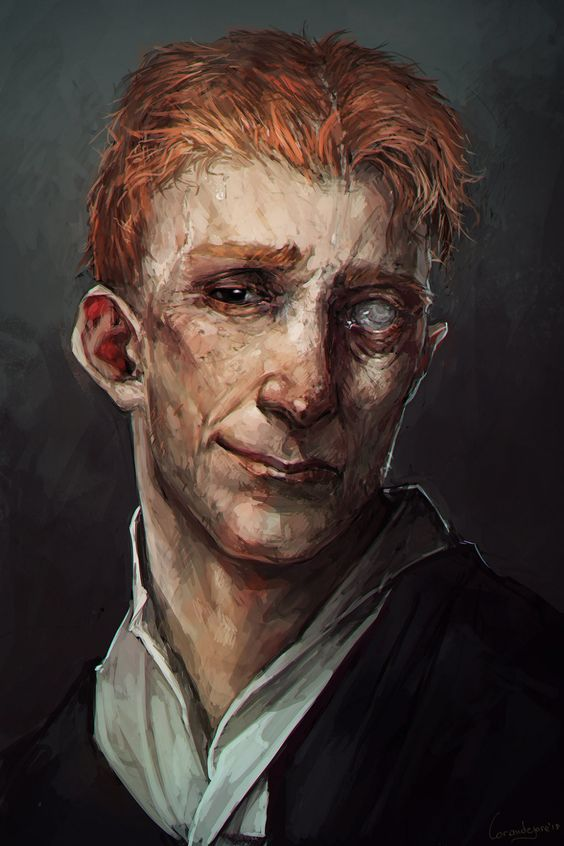
\includegraphics[width=0.2\textwidth]{img/harold}
    \end{center}
  \end{wrapfigure}
  \subsection {Harold "Scar" of Kremle}
  \paragraph{Heavy weapons fighter}
  Despite being a lyrist, he has an unusually muscular build and strong arms, almost as if the small instrument in his hand might accidentally be crushed. Clearly familiar with both the city and the wilderness, hard work is no stranger to him. An ugly scar on his face gives him a rather intimidating expression more fitting for a criminal than a wandering bard, even though his attire and rather joyous expression might suggest otherwise.


  \begin{wrapfigure}{r}{0.2\textwidth}
    \begin{center}
      
\includegraphics[width=0.2\textwidth]{img/yasmina}
    \end{center}
  \end{wrapfigure}
  \subsection{Yasmina}
  \paragraph{Divination Wizard}
  An enthusiastic human wizard, longing for adventure, who always wears a diadem on her forehead. She claims to have done forced labour because she refused a powerful lecherous nobleman, and her lawyer messed it up, turning her from a victim into a perpetrator. She seems to be very clever, not ugly either, and moves as gracefully as a cat, but they've never entrusted her with anything heavier than a broom. She is knowledgeable in history and magic and has occasionally saved someone from injury thanks to her visions.


  \begin{wrapfigure}{r}{0.2\textwidth}
    \begin{center}
      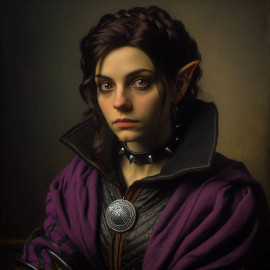
\includegraphics[width=0.2\textwidth]{img/silgrid}
    \end{center}
  \end{wrapfigure}
  \subsection{Silgrid Coalbraid}
  \paragraph{Dwarven rogue}
  A trusting, devout dwarf with a dark metal collar. She exudes compassion and understanding, but she might be a bit of a weirdo; I feel like she experiences other people's emotions too intensely. Unlike other dwarves, she's rather small and slender, probably wouldn't last long in the mines, but she moves quickly and has a good aim. She often discreetly prays in dark alleys when nobody's looking. She still wears a black clothes, and despite all her strange quirks, she's quite easy to talk to.


  \begin{wrapfigure}{r}{0.2\textwidth}
    \begin{center}
      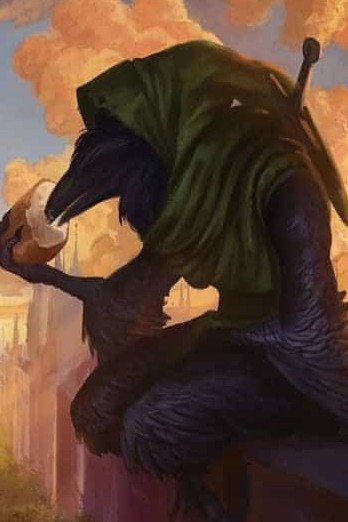
\includegraphics[width=0.2\textwidth]{img/sally}
    \end{center}
  \end{wrapfigure}
  \subsection{Sally “Jackdaw” Horst}
  \paragraph{Kenku ranger, druid fighting style}
  A secretive grey-black Kenku rumoured to have once been part of the city watch. Unable to speak, only mimics other voices and sounds. Not very strong, which isn't unusual for a bird-like race. Appears to act with caution and not be overly swayed by emotions. Moves calmly and carefully observes the surroundings, alert to every rustle. Seems to have a grasp of nature and remains unfazed by anything in the city. He values morality highly and despises all criminal activities.

  \pagebreak
\end{onecolumn}

\chapter{Section}

\DndDropCapLine{T}{his example is designed to aid you in} writing beautifully typeset documents for the fifth edition of the world's greatest roleplaying game. It starts by adjusting the section formatting from the defaults in \LaTeX{} to something a bit more familiar to the reader. The chapter formatting is displayed above.

\section{Section}
Sections break up chapters into large groups of associated text.

\subsection{Subsection}
Subsections further break down the information for the reader.

\subsubsection{Subsubsection}
Subsubsections are the furthest division of text that still have a block header. Below this level, headers are displayed inline.

\paragraph{Paragraph}
The paragraph format is seldom used in the core books, but is available if you prefer it to the ``normal'' style.

\subparagraph{Subparagraph}
The subparagraph format with the paragraph indent is likely going to be more familiar to the reader.

\section{Special Sections}
The module also includes functions to aid in the proper typesetting of multi-line section headers: |\DndFeatHeader| for feats, |\DndItemHeader| magic items and traps, and |\DndSpellHeader| for spells.

\DndFeatHeader{Typesetting Savant}[Prerequisite: \LaTeX{} distribution]
You have acquired a package which aids in typesetting source material for one of your favorite games. You have advantage on Intelligence checks to typeset new content. On a failed check, you can ask questions online at the package's website.

\DndItemHeader{Foo's Quill}{Wondrous item, rare}
This quill has 3 charges. While holding it, you can use an action to expend 1 of its charges. The quill leaps from your hand and writes a contract applicable to your situation.

The quill regains 1d3 expended charges daily at dawn.

\DndSpellHeader%
  {Beautiful Typesetting}
  {4th-level illusion}
  {1 action}
  {5 feet}
  {S, M (ink and parchment, which the spell consumes)}
  {Until dispelled}
You are able to transform a written message of any length into a beautiful scroll. All creatures within range that can see the scroll must make a wisdom saving throw or be charmed by you until the spell ends.

While the creature is charmed by you, they cannot take their eyes off the scroll and cannot willingly move away from the scroll. Also, the targets can make a wisdom saving throw at the end of each of their turns. On a success, they are no longer charmed.

\section{Map Regions}
The map region functions |\DndArea| and |\DndSubArea| provide automatic numbering of areas.

\DndArea{Village of Hommlet}
This is the village of hommlet.

\DndSubArea{Inn of the Welcome Wench}
Inside the village is the inn of the Welcome Wench.

\DndSubArea{Blacksmith's Forge}
There's a blacksmith in town, too.

\DndArea{Foo's Castle}
This is foo's home, a hovel of mud and sticks.

\DndSubArea{Moat}
This ditch has a board spanning it.

\DndSubArea{Entrance}
A five-foot hole reveals the dirt floor illuminated by a hole in the roof.

\chapter{Text Boxes}

The module has three environments for setting text apart so that it is drawn to the reader's attention. |DndReadAloud| is used for text that a game master would read aloud.

\begin{DndReadAloud}
  As you approach this module you get a sense that the blood and tears of many generations went into its making. A warm feeling welcomes you as you type your first words.
\end{DndReadAloud}

\section{As an Aside}
The other two environments are the |DndComment| and the |DndSidebar|. The |DndComment| is breakable and can safely be used inline in the text.

\begin{DndComment}{This Is a Comment Box!}
  A |DndComment| is a box for minimal highlighting of text. It lacks the ornamentation of |DndSidebar|, but it can handle being broken over a column.
\end{DndComment}

The |DndSidebar| is not breakable and is best used floated toward a page corner as it is below.

\begin{DndSidebar}[float=!b]{Behold the DndSidebar!}
  The |DndSidebar| is used as a sidebar. It does not break over columns and is best used with a figure environment to float it to one corner of the page where the surrounding text can then flow around it.
\end{DndSidebar}

\section{Tables}
The |DndTable| colors the even rows and is set to the width of a line by default.

\begin{DndTable}[header=Nice Table]{XX}
    \textbf{Table head}  & \textbf{Table head} \\
    Some value  & Some value \\
    Some value  & Some value \\
    Some value  & Some value
\end{DndTable}

\chapter{Monsters and NPCs}

% Monster stat block
\begin{DndMonster}[float*=b,width=\textwidth + 8pt]{Monster Foo}
  \begin{multicols}{2}
    \DndMonsterType{Medium aberration (metasyntactic variable), neutral evil}

    % If you want to use commas in the key values, enclose the values in braces.
    \DndMonsterBasics[
        armor-class = {9 (12 with \emph{mage armor})},
        hit-points  = {\DndDice{3d8 + 3}},
        speed       = {30 ft., fly 30 ft.},
      ]

    \DndMonsterAbilityScores[
        str = 12,
        dex = 8,
        con = 13,
        int = 10,
        wis = 14,
        cha = 15,
      ]

    \DndMonsterDetails[
        %saving-throws = {Str +0, Dex +0, Con +0, Int +0, Wis +0, Cha +0},
        %skills = {Acrobatics +0, Animal Handling +0, Arcana +0, Athletics +0, Deception +0, History +0, Insight +0, Intimidation +0, Investigation +0, Medicine +0, Nature +0, Perception +0, Performance +0, Persuasion +0, Religion +0, Sleight of Hand +0, Stealth +0, Survival +0},
        %damage-vulnerabilities = {cold},
        %damage-resistances = {bludgeoning, piercing, and slashing from nonmagical attacks},
        %damage-immunities = {poison},
        %condition-immunities = {poisoned},
        senses = {darkvision 60 ft., passive Perception 10},
        languages = {Common, Goblin, Undercommon},
        challenge = 1,
      ]
    % Traits
    \DndMonsterAction{Innate Spellcasting}
    Foo's spellcasting ability is Charisma (spell save DC 12, +4 to hit with spell attacks). It can innately cast the following spells, requiring no material components:
    \begin{DndMonsterSpells}
      \DndInnateSpellLevel{misty step}
      \DndInnateSpellLevel[3]{fog cloud, rope trick}
      \DndInnateSpellLevel[1]{identify}
    \end{DndMonsterSpells}

    \DndMonsterAction{Spellcasting}
    Foo is a 2nd-level spellcaster. Its spellcasting ability is Charisma (spell save DC 12, +4 to hit with spell attacks). It has the following sorcerer spells prepared:
    \begin{DndMonsterSpells}
      \DndMonsterSpellLevel{blade ward, fire bolt, light, shocking grasp}
      \DndMonsterSpellLevel[1][3]{burning hands, mage armor, shield}
    \end{DndMonsterSpells}

    \DndMonsterSection{Actions}
    \DndMonsterAction{Multiattack}
    The foo makes two melee attacks.

    %Default values are shown commented out
    \DndMonsterAttack[
      name=Dagger,
      %distance=both, % valid options are in the set {both,melee,ranged},
      %type=weapon, %valid options are in the set {weapon,spell}
      mod=+3,
      %reach=5,
      %range=20/60,
      %targets=one target,
      dmg=\DndDice{1d4+1},
      dmg-type=piercing,
      %plus-dmg=,
      %plus-dmg-type=,
      %or-dmg=,
      %or-dmg-when=,
      %extra=,
    ]

    %\DndMonsterMelee calls \DndMonsterAttack with the melee option
    \DndMonsterMelee[
      name=Flame Tongue Longsword,
      mod=+3,
      %reach=5,
      %targets=one target,
      dmg=\DndDice{1d8+1},
      dmg-type=slashing,
      plus-dmg=\DndDice{2d6},
      plus-dmg-type=fire,
      or-dmg=\DndDice{1d10+1},
      or-dmg-when=if used with two hands,
      %extra=,
    ]

    %\DndMonsterRanged calls \DndMonsterAttack with the ranged option
    \DndMonsterRanged[
      name=Assassin's Light Crossbow,
      mod=+1,
      range=80/320,
      dmg=\DndDice{1d8},
      dmg-type=piercing,
      %plus-dmg=,
      %plus-dmg-type=,
      %or-dmg=,
      %or-dmg-when=,
      extra={, and the target must make a DC 15 Constitution saving throw, taking 24 (7d6) poison damage on a failed save, or half as much damage on a successful one}
    ]

    % Legendary Actions
    \DndMonsterSection{Legendary Actions}
    The foo can take 3 legendary actions, choosing from the options below. Only one legendary action option can be used at a time and only at the end of another creature's turn. The foo regains spent legendary actions at the start of its turn.

    \begin{DndMonsterLegendaryActions}
      \DndMonsterLegendaryAction{Move}{The foo moves up to its speed.}
      \DndMonsterLegendaryAction{Dagger Attack}{The foo makes a dagger attack.}
      \DndMonsterLegendaryAction{Create Contract (Costs 3 Actions)}{The foo presents a contract in a language it knows and waves it in the face of a creature within 10 feet. The creature must make a DC 10 Intelligence saving throw. On a failure, the creature is incapacitated until the start of the foo's next turn. A creature who cannot read the language in which the contract is written has advantage on this saving throw.}
    \end{DndMonsterLegendaryActions}
  \end{multicols}
\end{DndMonster}

The |DndMonster| environment is used to typeset monster and NPC stat blocks. The module supplies many functions to easily typeset the contents of the stat block

\chapter{Colors}

\begin{table*}[b]%
  \caption{}\label{tab:colors}

  \begin{DndTable}[width=\linewidth,header=Colors Supported by This Package]{lX}
    \textbf{Color}                  & \textbf{Description} \\
    |PhbLightGreen|                 & Light green used in PHB Part 1 (Default) \\
    |PhbLightCyan|                  & Light cyan used in PHB Part 2 \\
    |PhbMauve|                      & Pale purple used in PHB Part 3 \\
    |PhbTan|                        & Light brown used in PHB appendix \\
    |DmgLavender|                   & Pale purple used in DMG Part 1 \\
    |DmgCoral|                      & Orange-pink used in DMG Part 2 \\
    |DmgSlateGray| (|DmgSlateGrey|) & Blue-gray used in PHB Part 3 \\
    |DmgLilac|                      & Purple-gray used in DMG appendix \\
  \end{DndTable}
\end{table*}

This package provides several global color variables to style |DndComment|, |DndReadAloud|, |DndSidebar|, and |DndTable| environments.

\begin{DndTable}[header=Box Colors]{lX}
  \textbf{Color}   & \textbf{Description} \\
  |commentcolor|   & |DndComment| background \\
  |readaloudcolor| & |DndReadAloud| background \\
  |sidebarcolor|   & |DndSidebar| background \\
  |tablecolor|     & background of even |DndTable| rows \\
\end{DndTable}

They also accept an optional color argument to set the color for a single instance. See Table~\ref{tab:colors} for a list of core book accent colors.

\begin{lstlisting}
\begin{DndTable}[color=PhbLightCyan]{cX}
  \textbf{d8} & \textbf{Item} \\
  1 & Small wooden button \\
  2 & Red feather \\
  3 & Human tooth \\
  4 & Vial of green liquid \\
  6 & Tasty biscuit \\
  7 & Broken axe handle \\
  8 & Tarnished silver locket \\
\end{DndTable}
\end{lstlisting}

\begin{DndTable}[color=PhbLightCyan]{cX}
  \textbf{d8} & \textbf{Item} \\
  1 & Small wooden button \\
  2 & Red feather \\
  3 & Human tooth \\
  4 & Vial of green liquid \\
  6 & Tasty biscuit \\
  7 & Broken axe handle \\
  8 & Tarnished silver locket \\
\end{DndTable}

\section{Themed Colors}
Use |\DndSetThemeColor[<color>]| to set |commentcolor|, |readaloudcolor|, |sidebarcolor|, and |tablecolor| to a specific color. Calling |\DndSetThemeColor| without an argument sets those colors to the current |themecolor|. In the following example the group limits the change to just a few boxes; after the group finishes, the colors are reverted to what they were before the group started.

\begin{lstlisting}
\begingroup
\DndSetThemeColor[PhbMauve]

\begin{DndComment}{This Comment Is in Mauve}
  This comment is in the the new color.
\end{DndComment}

\begin{DndSidebar}{This Sidebar Is Also Mauve}
  The sidebar is also using the new theme color.
\end{DndSidebar}
\endgroup
\end{lstlisting}

\begingroup
\DndSetThemeColor[PhbMauve]

\begin{DndComment}{This Comment Is in Mauve}
  This comment is in the the new color.
\end{DndComment}

\begin{DndSidebar}{This Sidebar Is Also Mauve}
  The sidebar is also using the new theme color.
\end{DndSidebar}
\endgroup

\end{document}
